\documentclass[12pt, a4paper]{article}
\usepackage[margin=1.5in]{geometry}
\usepackage{graphicx}
\usepackage{amsmath}
\usepackage{float}
\usepackage{listings}
\usepackage[shortlabels]{enumitem}


\setlength\parindent{0pt}
\newcommand{\code}{\lstinline[basicstyle=\small]}
\lstset{
    language=Python,
    basicstyle=\scriptsize
}


\title{EE2703: Applied Programming Lab \\ \Large Assignment 4: Fourier Approximations}
\author{Soham Roy \\ \normalsize EE20B130}
\date{\today}
\begin{document}

\maketitle % Insert the title, author and date


\section{Introduction}
Two functions, $exp(x)$ and $cos(cos(x))$ over the interval $[0,2\pi)$ will be modeled using
the fourier series:
\begin{equation*}
    a_0 + \sum_{n=1}^{\infty} \{a_n \cos(nx) + b_n \sin(nx)\}
\end{equation*}
Where,
\begin{align*}
    a_0 & = \frac{1}{2\pi} \int_{0}^{2\pi} f(x) dx       \\
    a_n & = \frac{1}{\pi} \int_{0}^{2\pi} f(x)cos(nx) dx \\
    a_n & = \frac{1}{\pi} \int_{0}^{2\pi} f(x)sin(nx) dx \\
\end{align*}
\pagebreak


\section{Subquestions}
\subsection{Define \& Plot Python Functions}
Two Python functions are defined:

% \par\rule{\linewidth}{0.4pt}
\begin{lstlisting}
    def exp(x):  # exponential function, supports value or vector
        return np.exp(x)

    def coscos(x):  # cos of cos function, supports value or vector
        return np.cos(np.cos(x))
\end{lstlisting}
% \par\rule[1.5ex]{\linewidth}{0.4pt}

The functions have been plotted with their periodic extensions ($2\pi$ period):
\begin{figure}[H]
    \centering
    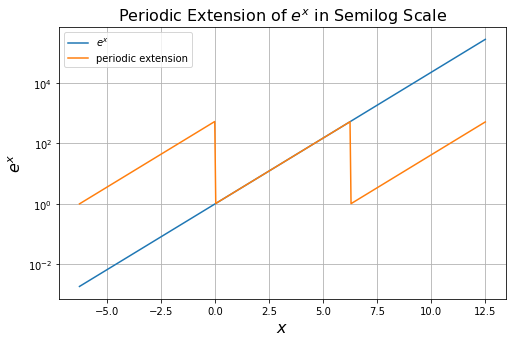
\includegraphics[scale=0.6]{1a.png}
\end{figure}
\begin{figure}[H]
    \centering
    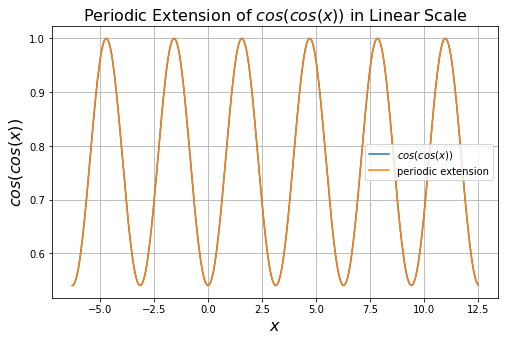
\includegraphics[scale=0.6]{1b.png}
\end{figure}
\pagebreak


\subsection{Evaluate Integrals}
The integrands have been defined as functions of \code{x}, \code{k}, and \code{f}, where
\code{f} is the Python function to be approximated, i.e. \code{exp} or \code{coscos}:
\begin{lstlisting}
    def u(x, k, f):  # f is either exp or coscos
        return f(x) * np.cos(k * x)

    def v(x, k, f):  # f is either exp or coscos
        return f(x) * np.sin(k * x)
\end{lstlisting}
The integrals to calculate the values of $a_n$ and $b_n$ have been evaluated using the following loop:
\begin{lstlisting}
    F = [exp, coscos]
    a_0 = np.zeros((2))
    a_n = np.zeros((2, 25))
    b_n = np.zeros((2, 25))

    for i in range(2):  # iterate over exp and coscos
        a_0[i] = quad(F[i], 0, 2 * np.pi)[0] / (2 * np.pi)

    for j in range(25):  # integration
        a_n[i, j] = quad(u, 0, 2 * np.pi, args=(j + 1, F[i]))[0] / np.pi
        b_n[i, j] = quad(v, 0, 2 * np.pi, args=(j + 1, F[i]))[0] / np.pi
\end{lstlisting}


\subsection{Plot the Fourier Coefficients}
The answer vector $c$ has been generated by:
\begin{lstlisting}
    c_n = np.zeros((2, 51))  # c_n[0] and c_n[1] are the answer vectors
    c_n[:, 0] = a_0
    c_n[:, 1::2] = a_n  # alternate elements starting at 1
    c_n[:, 2::2] = b_n  # alternate elements starting at 2    
\end{lstlisting}

To plot in semilog scale, for example, we use:
\begin{lstlisting}
    plt.semilogy(0, np.abs(a_0[f_i]), 'ro', label="by integration")
    plt.semilogy(range(1, 26), np.abs(a_n[f_i]), 'ro')
    plt.semilogy(range(1, 26), np.abs(b_n[f_i]), 'ro')
\end{lstlisting}

The coefficients $|a_n|$ and $|b_n|$ have been plotted:
\begin{figure}[H]
    \centering
    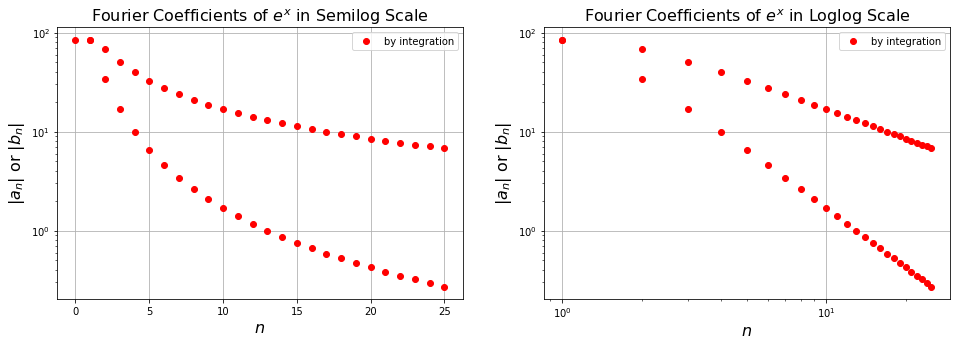
\includegraphics[scale=0.39]{3a.png}
\end{figure}
\begin{figure}[H]
    \centering
    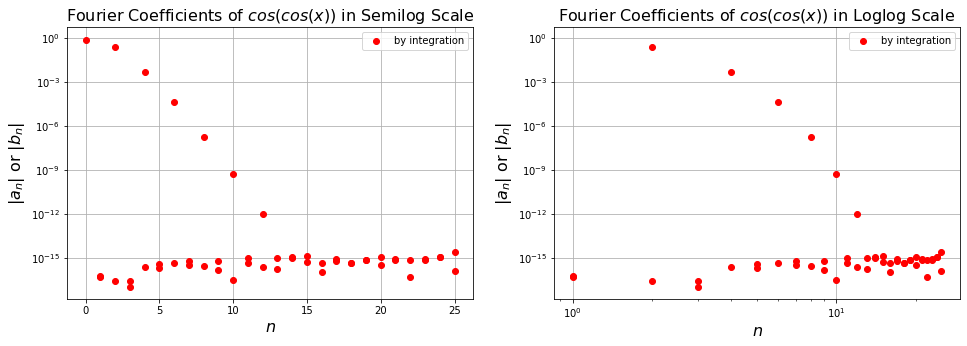
\includegraphics[scale=0.39]{3b.png}
\end{figure}


\begin{enumerate}[(a)]
    \item The $b_n$ coefficients for $cos(cos(x))$ are of the order of magnitude $-16$, i.e. nearly zero. \\
          This is because $cos(cos(x))$ is an even function, and thus does not have any odd component.
    \item $cos(cos(x))$ is a periodic function, comprising not many frequencies. \\
          $e^x$, on the other hand, is a non-periodic function, and thus its periodic extension has multiple
          discontinuities. Hence, high frequency components are required to represent this function as a sum
          of trigonometric functions.
    \item The $loglog$ plot is linear for $e^x$ because the $log$ of its coefficients vary linearly with
          $log(n)$, i.e. the coefficients depend on $\frac{1}{n^a}$ for some $a$. \\
          On the other hand, the $semilog$ plot is linear for $cos(cos(x))$ because the $log$ of its
          coefficients vary linearly with $n$, i.e. the coefficients decay exponentially.
\end{enumerate}


\subsection{Least Squares}
The equation to be solved by \code{scipy.linalg.lstsq} is:
\begin{equation*}
    Ac = B
\end{equation*}

The matrix $A$ has been generated by:
\begin{lstlisting}
    A = np.ones((400, 51))  # first column should be ones
    for k in range(1, 26):
        A[:, 2 * k - 1] = np.cos(k * x)
        A[:, 2 * k] = np.sin(k * x)
\end{lstlisting}

The solution matrices are \code{c[0]} for $e^x$ and
\code{c[1]} for $coscos(x)$:
\begin{lstlisting}
    for i in range(2):
        b = F[i](x)
        c[i] = lstsq(A, b)[0]
\end{lstlisting}


\subsection{Plot the Best Fit Coefficients}
To plot in semilog scale, for example, we use:
\begin{lstlisting}
    plt.semilogy(0, np.abs(c[f_i][0]), 'go', label="by least squares")
    plt.semilogy(range(1, 26), np.abs(c[f_i][1::2]), 'go')
    plt.semilogy(range(1, 26), np.abs(c[f_i][2::2]), 'go')
\end{lstlisting}

The coefficients $|a_n|$ and $|b_n|$ by least squares method have been contrasted with
those by integration:
\begin{figure}[H]
    \centering
    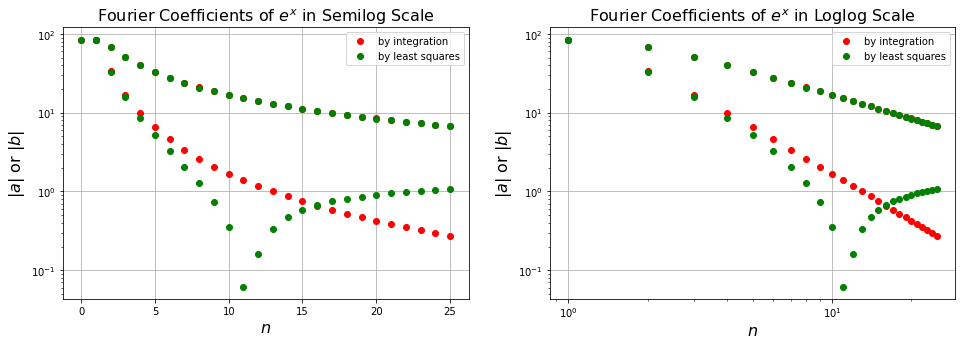
\includegraphics[scale=0.39]{5a.png}
\end{figure}
\begin{figure}[H]
    \centering
    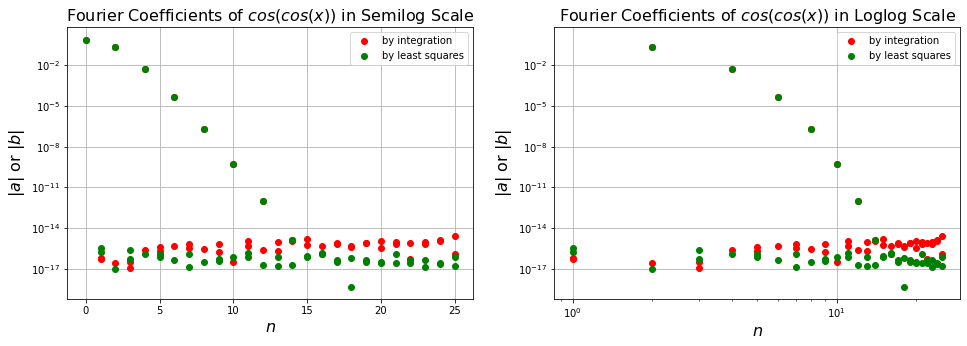
\includegraphics[scale=0.39]{5b.png}
\end{figure}


\subsection{Compare Least Squares and Direct Integration}
The maximum errors between the least squares and direct integration methods has been calculated:
\begin{lstlisting}
    np.max(np.abs(c[0] - c_n[0]))  # for e^x
    np.max(np.abs(c[1] - c_n[1]))  # for coscos(x)
\end{lstlisting}

\begin{tabular}{lcl}
    The largest deviation of coefficients for & $e^x$         & is : 1.3327     \\
    The largest deviation of coefficients for & $cos(cos(x))$ & is : 2.6684e-15
\end{tabular}
\medskip

The error is significant for $e^x$ but negligible for $cos(cos(x))$. \\
This is because there are multiple discontinuities in the periodic extension of $e^x$, and thus
would require a much higher number of coefficients to be somewhat accurately represented. \\
This lack in accuracy is more apparent close to those discontinuities.

\subsection{Plot the Fourier Approximations}
The functions as represented by the Fourier coefficients calculated through the least squares method
have been plotted:
\begin{lstlisting}
    plt.plot(x[200:600], np.dot(A, c[1]), 'go', label="by least squares")
\end{lstlisting}
\begin{figure}[H]
    \centering
    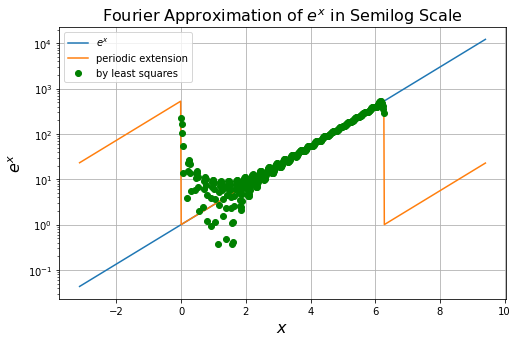
\includegraphics[scale=0.6]{7a.png}
\end{figure}
\begin{figure}[H]
    \centering
    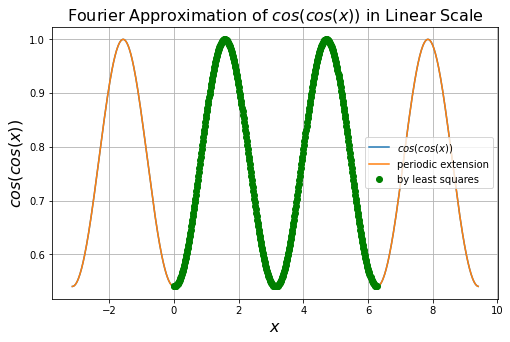
\includegraphics[scale=0.6]{7b.png}
\end{figure}

The $cos(cos(x))$ plot agrees nearly perfectly, but the $e^x$ plot has a large deviation.
This is because unlike $cos(cos(x))$, which has periodic components, the $e^x$ function
is not inherently comprised of periodic trigonometric functions. The periodic extension of $e^x$
has multiple discontinuities, which causes the Fourier representation to overshoot around them
due to the Gibbs phenomenon.



\end{document}
